\chapter{データ} 

\section{SDO / AIA}
モデルの学習及び評価データとして、NASAのSolar Dynamic Observatory(SDO)(\cite{pesnell2012solar})のAtmospheric Imaging Assembly(AIA)(\cite{lemen2012atmospheric})で撮影された紫外線観測データを用いた。

SDOはNASAのLiving With a Star(LWS)プログラムの一つとして2010年2月に打ち上げられた太陽観測衛星である。
AIA、Helioseismic and Magnetic Imager(HMI)、Extreme Ultraviolet Variability Experiment(EVE)などの高い空間解像度、時間分解能を持つ観測機器を搭載し、地上では不可能な多くの波長でのデータを提供する。
その観測データを用いることにより、太陽物理学、宇宙天気、また地球環境に関する理解や洞察を深めることが期待されている。

AIAは主に太陽大気を観測する観測機器であり、4つの望遠鏡で構成されている。
また、7つの極紫外線フィルターと、2つの紫外線フィルター、および1つの可視光フィルターを持ち、広範な温度帯で太陽大気を観察することを可能にしている。
本研究で用いられる171Å、193Å、211Åの3つのフィルターは、36秒間隔で撮影され、4096×4096、約1.5秒角の空間解像度を持つ

これらのデータはJoint Science Operations Center(JSOC) によって提供されており、Pythonの太陽物理学を支援するライブラリであるSunpyを用いてダウンロードすることができる。


\subsection{AIA 211Å}
    表\ref{table:aia_filters_details}のように、211Å( 21.1 nm )のフィルターは、約200万Kの14価鉄(Fe XIV)イオンが放射するスペクトルを捉えるために特化している。
    この波長での観測は、活動領域のコロナを観測するのに最適である。図\ref{fig:sample_aia211}は、これらの特性を示している。

    \begin{figure}[h]
        \centering
        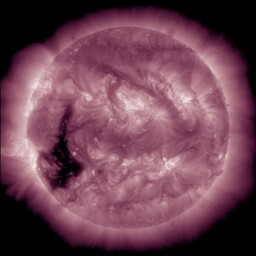
\includegraphics[width=0.8\textwidth]{figures/data/latest_256_0211.jpg}
        \caption{SDO/AIAの211Åフィルターで撮影された太陽全球紫外線像。強調のために紫色に色付けされている。球面の中上部から中下部には明るく輝く活動領域が見られ、左下部に暗くコロナホールが観測できる。}
        \label{fig:sample_aia211}
    \end{figure}

\subsection{AIA 193Å}
    表\ref{table:aia_filters_details}のように、193Å( 19.3 nm )のフィルターは、約150万Kの12価鉄(Fe XII)イオンが放射するスペクトル、または約2000万Kの24価鉄(Fe XXIV)イオンが放射するスペクトルを捉えるために特化している。
    前者は主にコロナの中程度の高温領域を観測するために用いられ、後者は、主にコロナの高温フレアプラズマを観測するために用いられる。さらに、コロナホールも強調して観測することができる。
    図\ref{fig:sample_aia193}は193Åフィルターで捉えた太陽像を示している。
    
    \begin{figure}[h]
        \centering
        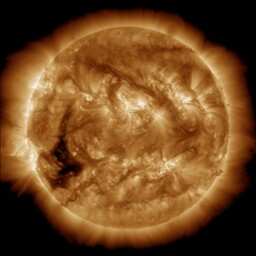
\includegraphics[width=0.8\textwidth]{figures/data/latest_256_0193.jpg}
        \caption{SDO/AIAの193Åフィルターで撮影された太陽全球紫外線像。強調のために橙色に色付けされている。}
        \label{fig:sample_aia193}
    \end{figure}
    
\subsection{AIA 171Å}
    表\ref{table:aia_filters_details}のように、171Å( 17.1 nm )のフィルターは、約60万Kの9価鉄(Fe IX)イオンが放射するスペクトルを捉えるために特化している。
    この波長での観測は、太陽のコロナループ、静穏領域コロナ、コロナホールなどの磁気構造を詳細に観察することができる。
    図\ref{fig:sample_aia171}に示される171Åフィルターによる観測は、これらの特徴を捉えている。
    
    \begin{figure}[h]
        \centering
        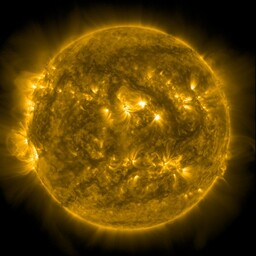
\includegraphics[width=0.8\textwidth]{figures/data/latest_256_0171.jpg}
        \caption{SDO/AIAの171Åフィルターで撮影された太陽全球紫外線像。強調のために黄色に色付けされている。193Å、211Åでは観察できない、コロナホールなどの静穏領域のスペクトルも観測できる。}
        \label{fig:sample_aia171}
    \end{figure}

\begin{table}[hptb]
    \centering
    \caption{SDO AIAの171, 193, 211(\AA)の特性}
    \begin{tabular}{lccc}
    \hline
    \textbf{フィルター (\AA)} & \textbf{主要イオン} & \textbf{観測される主要な太陽活動または領域} & \textbf{温度帯(K)}  \\ \hline
    171 & Fe IX & 静穏領域コロナ, 上層遷移領域 & \(6.3 \times 10^{5} \) \\ \hline
    193 & Fe XII, XXIV & コロナと高温フレアプラズマ & \(1.5 \times 10^6, 2.0 \times 10^7 \)  \\ \hline
    211 & Fe XIV & 活動領域コロナ & \(2.0 \times 10^6\) \\ \hline
    \end{tabular}
    \label{table:aia_filters_details}
\end{table}


\section{前処理}

本研究で用いるデータセットには、SDO/AIAのデータが提供されている2010年5月から、2022年10月までのデータが含まれている。  
この期間に存在するデータから、4時間ごとにデータを抽出し、各波長ごとに約22000枚をデータセットに含んでいる。
データはJSOCにより提供されているものをダウンロードし、その後、不正な画像を除去し、正規化やスケーリングを行った後、学習用、検証用、テスト用に分割した。
この手順をアルゴリズム\ref{alg:dataset_creation}に示す。
これらのデータを、24枚の画像を1セットとして分割する。各セットは24枚の時系列に並んだ画像で構成され、太陽全球の空間的情報の時間的変化を捉えている。
24枚のうち、前半の12枚、すなわち48時間までを入力シークエンス 、後半の12枚、すなわち52時間から96時間までを出力シークエンスとして扱う。
学習の際は、入力シークエンスに対して出力シークエンスを教師データとして扱い、テストの際は入力シークエンスに続くモデルにとって未知の出力シークエンスを再現できるか検証する。

このデータセットは第24太陽活動周期の初期から、第25周期の初期までの観測データを網羅している。この時間範囲には、太陽活動の活発性が高いフェーズと低いフェーズの両方が含まれている。従って、このデータセットは太陽活動の活発性に依存しない可能性が高く、その汎化能力に対する期待が一定程度裏付けられる。

\begin{algorithm}
    \caption{データセット作成アルゴリズム}
    \label{alg:dataset_creation}
    \begin{algorithmic}[1]
    \Procedure{CreateSolarDataset}{}
        \For{each wavelength in wavelengths}
            \State $images \gets \Call{DownloadData}{wavelength}$
            \State $images \gets \Call{ValidateAndReplaceImages}{images}$
            \State $all\_images.extend(images)$
        \EndFor
        \State $dataset \gets \Call{CreateDataset}{all\_images}$
        \State $processed\_dataset \gets \Call{PreprocessDataset}{dataset}$
        \State $train, val, test \gets \Call{SplitDataset}{processed\_dataset}$
        \State \Return $train, val, test$
    \EndProcedure
    
    \Function{DownloadData}{wavelength}
        \State \textit{Download data for given wavelength}
        \State \Return $images$
    \EndFunction
    
    \Function{ValidateAndReplaceImages}{images}
        \For{each image in images}
            \If{\textbf{not} \Call{ValidateImage}{image}}
                \State $alternative \gets \Call{FindAlternativeImage}{image.timestamp}$
                \State $images.replace(image, alternative)$
                \State \Call{ValidateAndReplaceImages}{images} \Comment{Recursive call}
            \EndIf
        \EndFor
        \State \Return $images$
    \EndFunction
    
    \Function{CreateDataset}{images}
        \State \textit{Create dataset by grouping 24 images}
        \State \Return $dataset$
    \EndFunction
    
    \Function{PreprocessDataset}{dataset}
        \State \textit{Apply preprocessing to each image in dataset}
        \State \Return $processed\_dataset$
    \EndFunction
    
    \Function{SplitDataset}{dataset}
        \State \textit{Split the dataset into train, validation, and test sets}
        \State \Return $train, val, test$
    \EndFunction
    \end{algorithmic}
\end{algorithm}

\subsection{不正な画像の除去}
SDO/AIA望遠鏡で撮影された全球画像には、露光時間が他の画像より極端に低い、画像内に太陽全体を捉えていない、などの不正な画像が含まれている。
確認することができた主な不正な画像を図\ref{fig:bad_aia_samples}に示す。

\begin{figure}[htbp]
    \centering
    \begin{subfigure}[b]{0.48\textwidth}
        
\includegraphics[width=\textwidth]{figures/data/bad_sample0.png}
        \caption{短い露光時間により、極端に暗い画像。}
    \end {subfigure}
    \hfill
    \begin{subfigure}[b]{0.48\textwidth}
        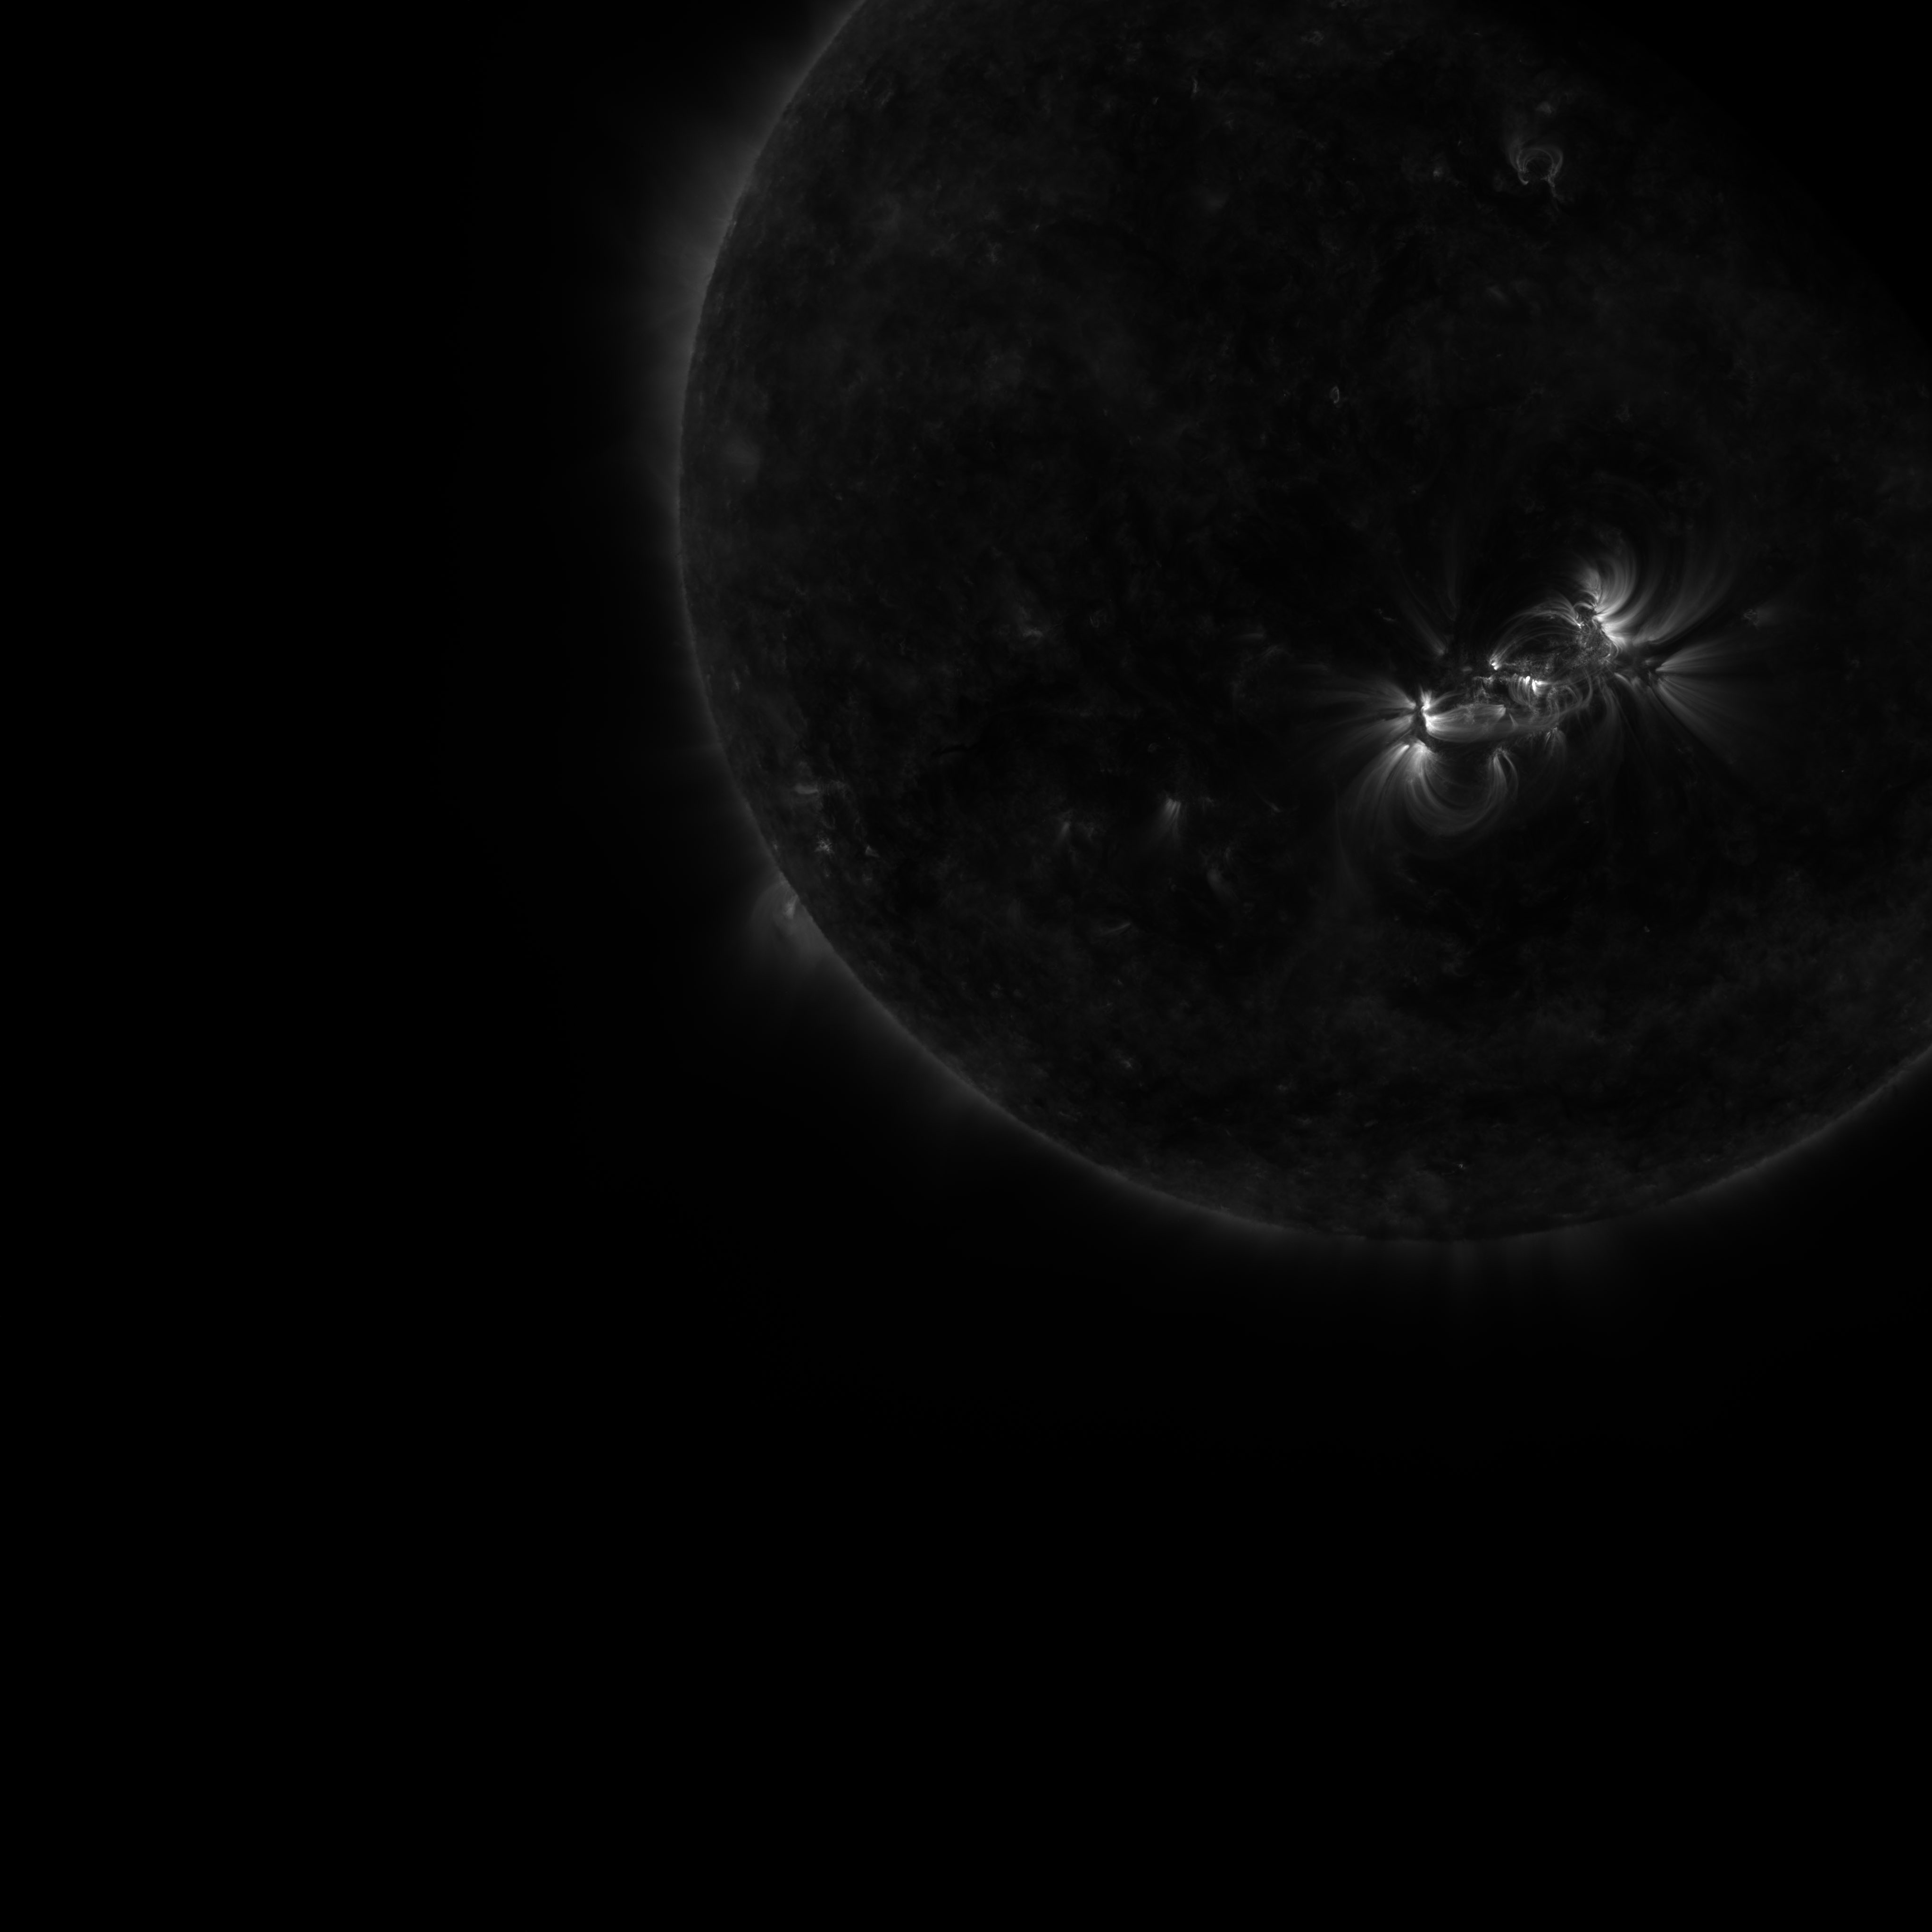
\includegraphics[width=\textwidth]{figures/data/bad_sample1.jpg}
        \caption{太陽が画像の中心にない画像。}
    \end {subfigure}
    \begin{subfigure}[b]{0.48\textwidth}
        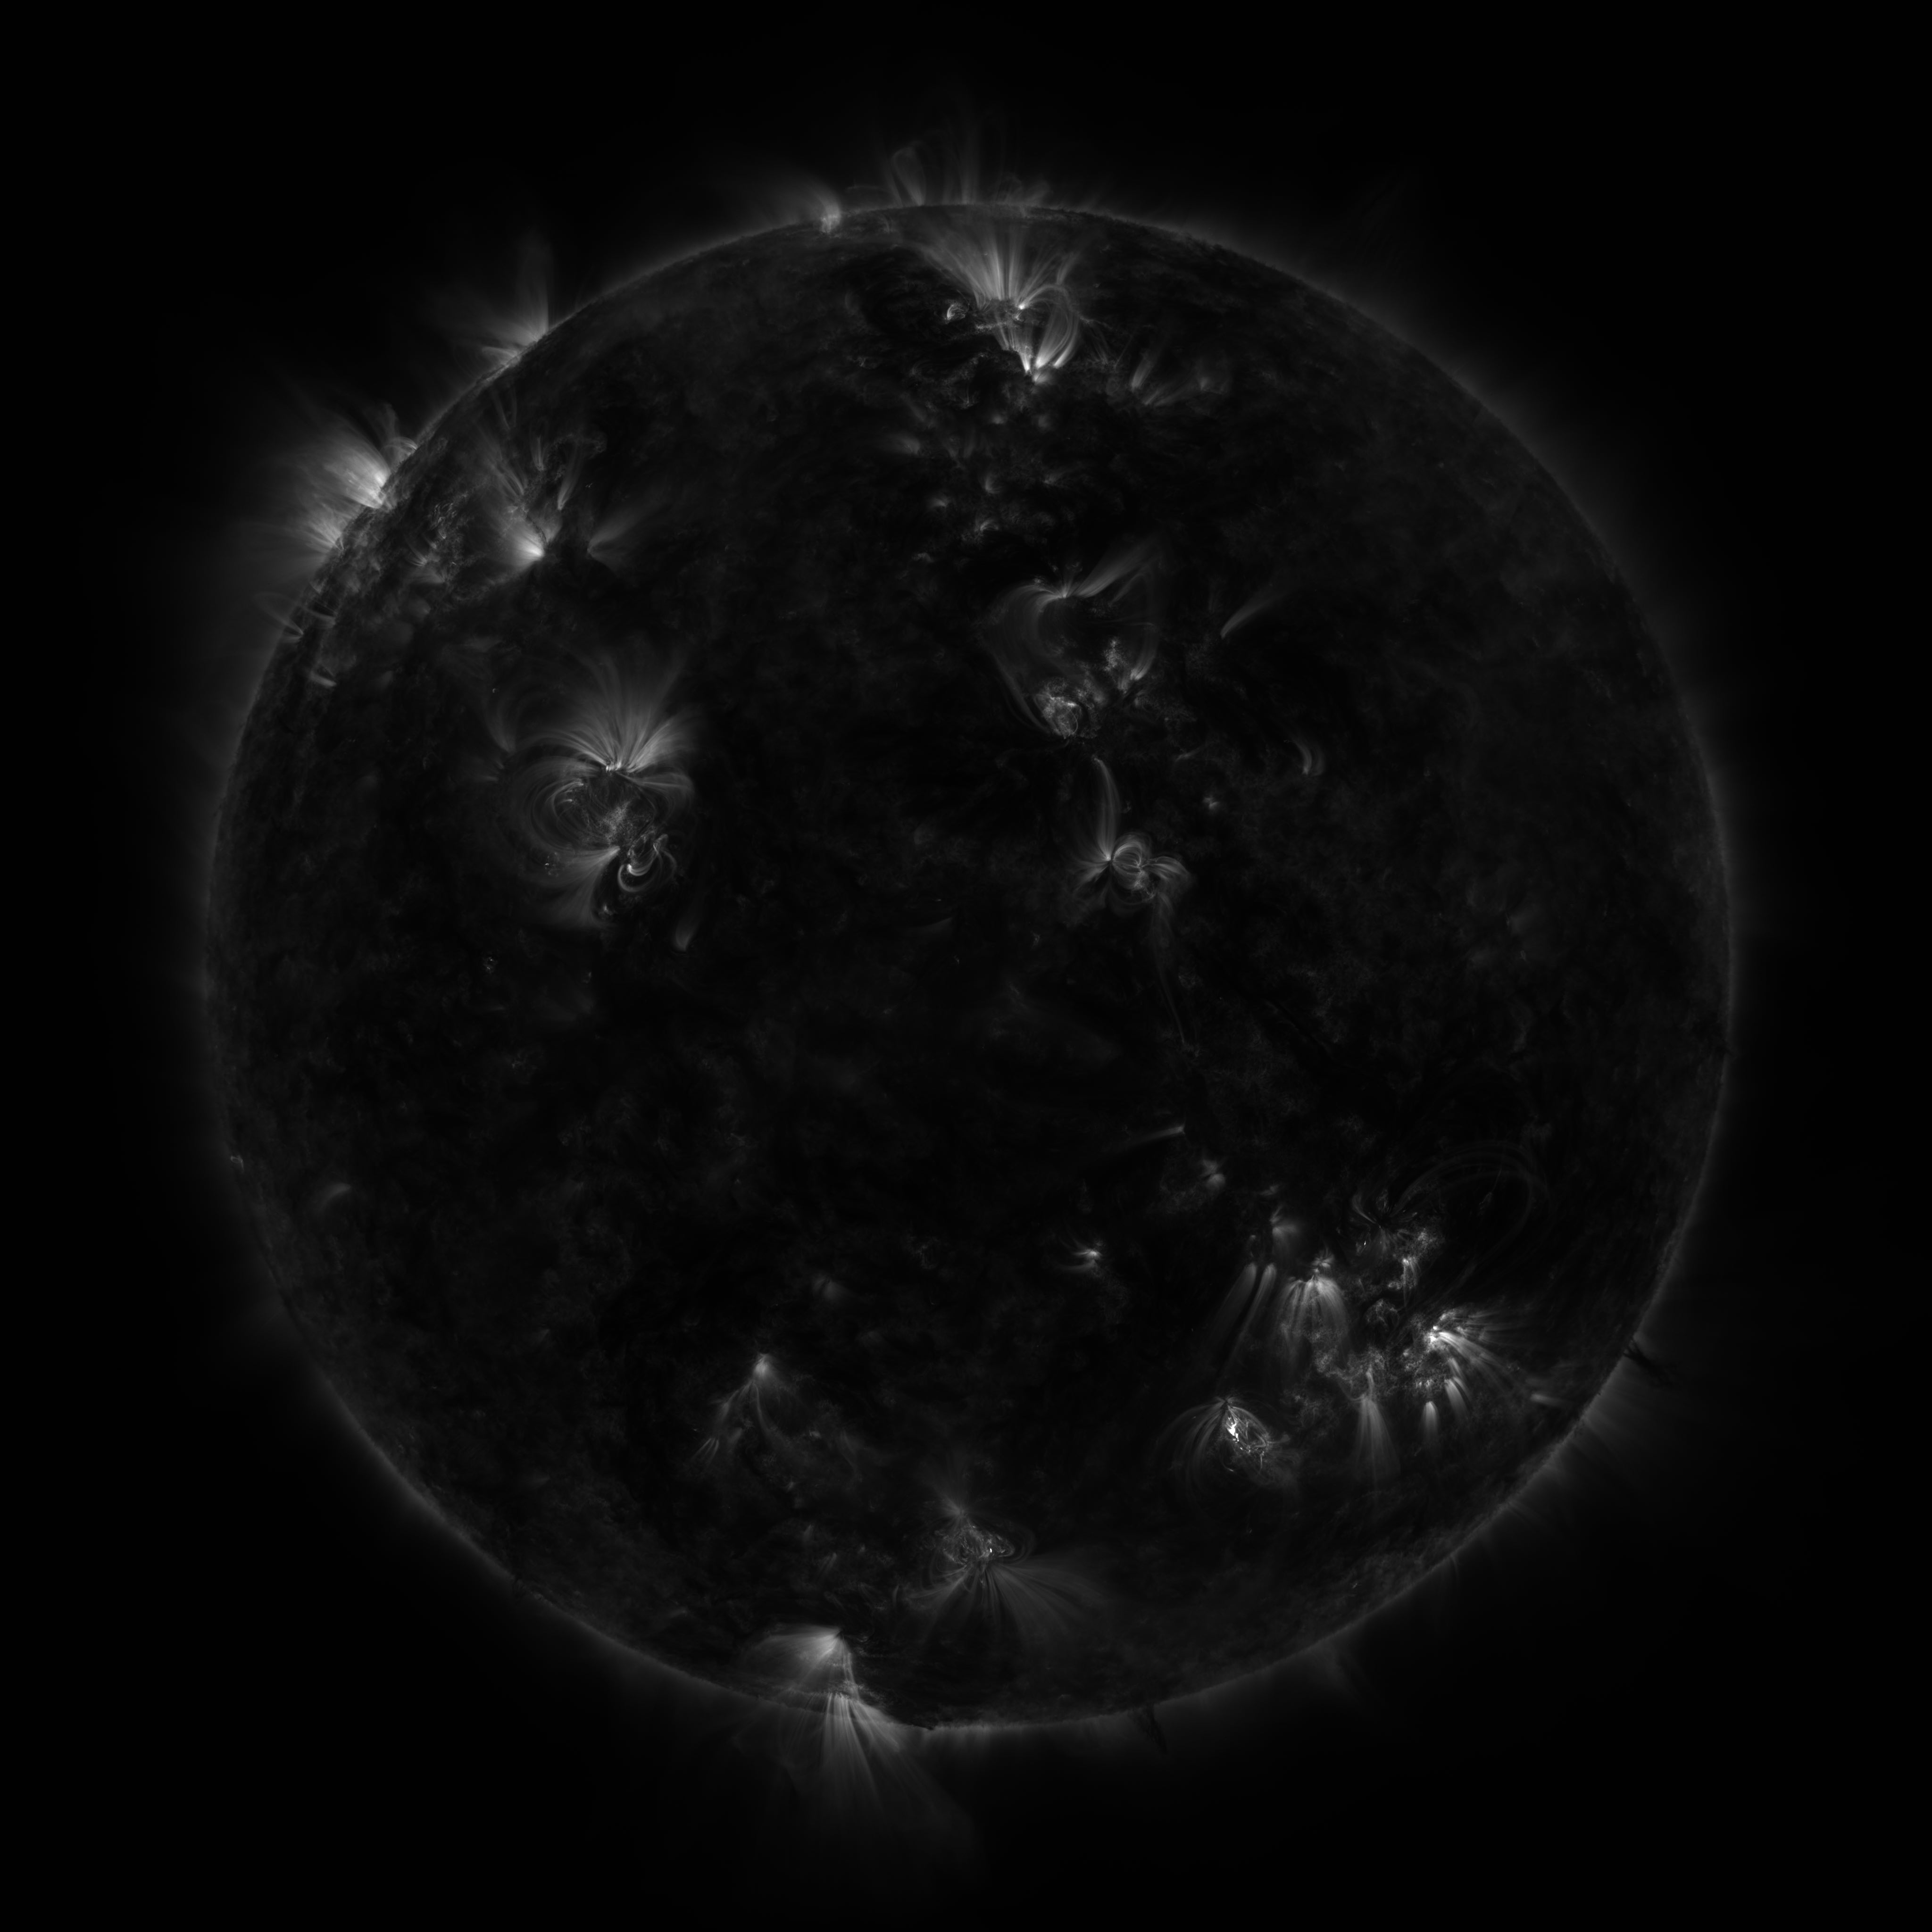
\includegraphics[width=\textwidth]{figures/data/bad_sample2.jpg}
        \caption{衛星が回転しており、正しい角度で太陽が撮影されていない画像。活動領域の少ない左下部と右上部が極である。}
    \end {subfigure}
    \hfill
    \caption{SDO/AIAにより観測された不正な画像の例}
    \label{fig:bad_aia_samples}
\end{figure}

これらの画像は、モデルの学習に悪影響を及ぼす可能性があるため、データセットから除去した。
機械学習のタスクによっては、十分なデータセットがあれば、モデルが不正な画像に対する頑健性を獲得し、不正な画像がデータセットに含まれていても、学習結果にあまり大きな影響を与えない場合がある。
しかし、本研究で行う動画予測は、データセットに含まれる画像がそのまま教師データとなるため、不正な画像は損失関数の計算、またはモデルの評価に大きな影響を与えるため、慎重に除去する必要がある。
データの除去には、FITSファイルのヘッダーに記録された各キーワードの値に対して閾値を設定して判定したのち、numpyによる輪郭検出を用いた月蝕判定関数により不正な画像を排除した。

\subsection{スケーリングと正規化}
    太陽動画データセットの前処理として、以下のステップを実施する。

    1. \textbf{正規化}: クリッピング処理されたデータを0から1の範囲に正規化する。ここで、ノイズによる負の値を削除し、極端に大きい外れ値の影響を削減するために、画像内の全ピクセル値に対して最小値を0、最大値を10000に設定した:
       \begin{equation}
       I_{normalized}(x, y) = \frac{min(max(I(x,y), 0), 10000)}{10000}
       \end{equation}

    2. \textbf{平方根スケーリング}: ダイナミックレンジの広さに対応するために、正規化されたデータに平方根スケーリングを適用する。この過程は以下の式で示される。
       \begin{equation}
       I_{scaled}(x, y) = \sqrt{I_{normalized}(x, y)}
       \end{equation}
        図\ref{fig:scale_histogram}のヒストグラムに示すように、スケーリングが適用されていないデータ(左)は、下位5\%程度の範囲に極端に輝度が集中している。平方根スケーリングを適用したデータ(右)では、そのような極端な輝度の差が緩和されている。

    \begin{figure}[htbp]
        \centering
        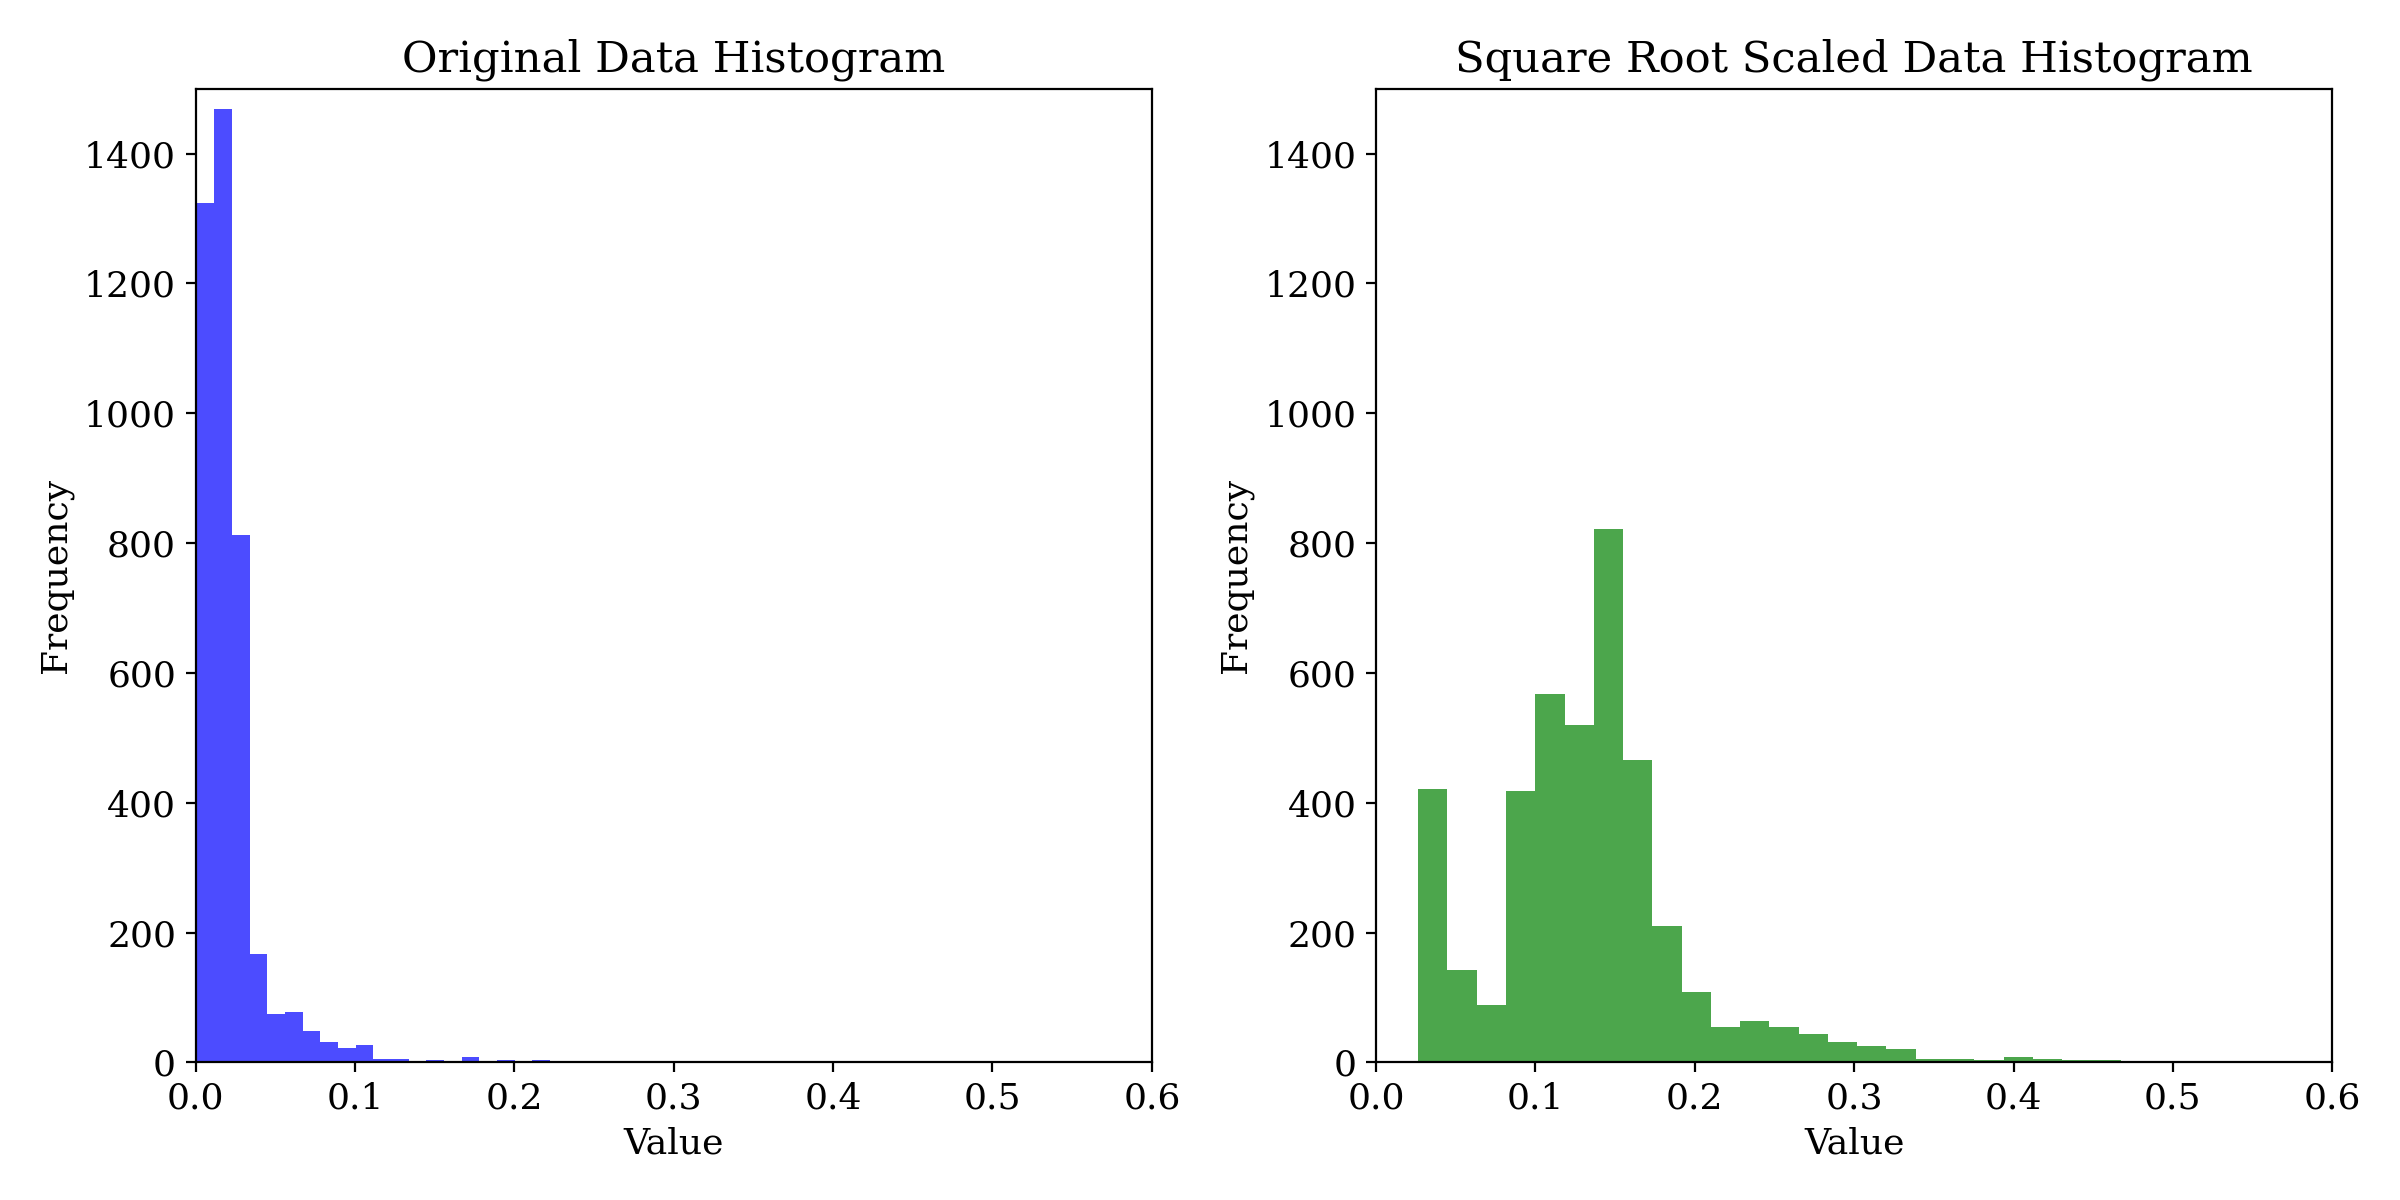
\includegraphics[width=\linewidth]{figures/data/histogram.png}
        \caption{ある画像での正規化されたデータに対する平方根スケーリングの効果。左: 正規化されたデータのヒストグラム。右: 平方根スケーリングを適用したデータのヒストグラム。}
        \label{fig:scale_histogram}
    \end{figure}

    3. \textbf{リサイズ}: 効率的な処理のために、$4192\text{px} \times 4192\text{px}$ の画像を$512\text{px} \times 512\text{px}$の解像度にリサイズした。この処理は、画像の空間解像度を低下させるが、太陽全球の大規模な構造を捉えるには十分である。


\subsection{データセットの分割}
このようにして作成されたデータセットは、約1000セットになり、これを学習用データセットに約800セット、検証データセットに50セット,テストデータセットに50セットというように分割した。
データセット1単位は、24枚の画像から構成される。

実験1では、211Åフィルターの画像のみを用いた。実験2では、171Å、193Å、211Åの3つのフィルターの画像を用いた。
最終的な分割とデータセットの概要を表\ref{tab:dataset}に示す。

\begin{table}[h]
    \centering
    \begin{tabular}{l|c|c}
    \hline
    実験 & 実験1 & 実験2 \\
    \hline\hline
    入力波長 & 211Å & 171Å,193Å,211Å \\
    \hline
    出力波長 & \multicolumn{2}{c}{211Å} \\
    \hline
    総枚数 & 22000 & 66000 \\
    \hline
    セット数 & \multicolumn{2}{c}{約1000} \\
    \hline
    セットごとの枚数 & \multicolumn{2}{c}{入力12 → 出力12} \\
    \hline
    解像度 & \multicolumn{2}{c}{512 * 512} \\
    \hline
    \end{tabular}
    \caption{各実験でのデータセット}
    \label{tab:dataset}
\end{table}
